\subsubsection{High-Pass Filter}

As the low-pass filter, the high-pass filter (e.g. is in Figure \ref{fig:high-pass})
has been realized on top of the FFT Filter,
in fact, it is the opposite to low-pass filter, and filters out
frequencies before 2853 Hz. What would be very useful to do is
to test it along with high-frequency boost, but we've never managed
to do so for 0.2.0.

\begin{figure}
	\centering
	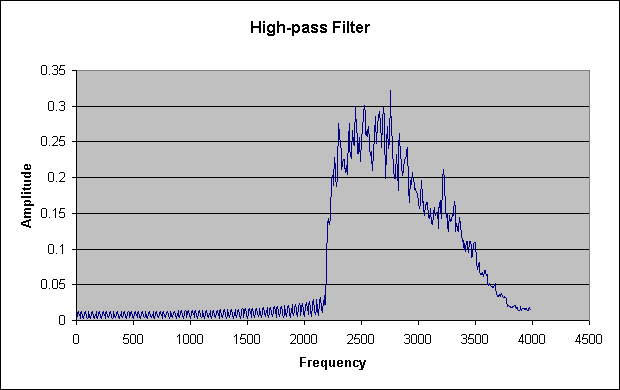
\includegraphics[width=400pt]{../graphics/graphs/high-pass-filter.png}
	\caption{High-pass filter applied to aihua5.wav.}
	\label{fig:high-pass}
\end{figure}
